\documentclass[]{book}

%These tell TeX which packages to use.
\usepackage{array,epsfig}
\usepackage{amsmath}
\usepackage{amsfonts}
\usepackage{amssymb}
\usepackage{amsxtra}
\usepackage{amsthm}
\usepackage{mathrsfs}
\usepackage{color}
\usepackage{pgfplots}

%Here I define some theorem styles and shortcut commands for symbols I use often
\theoremstyle{definition}
\newtheorem{defn}{Definition}
\newtheorem{thm}{Theorem}
\newtheorem{cor}{Corollary}
\newtheorem*{rmk}{Remark}
\newtheorem{lem}{Lemma}
\newtheorem*{joke}{Joke}
\newtheorem{ex}{Example}
\newtheorem*{soln}{Solution}
\newtheorem{prop}{Proposition}

\newcommand{\lra}{\longrightarrow}
\newcommand{\ra}{\rightarrow}
\newcommand{\surj}{\twoheadrightarrow}
\newcommand{\graph}{\mathrm{graph}}
\newcommand{\bb}[1]{\mathbb{#1}}
\newcommand{\B}{\mathrm{B}}
\newcommand{\Z}{\bb{Z}}
\newcommand{\Q}{\bb{Q}}
\newcommand{\R}{\bb{R}}
\newcommand{\C}{\bb{C}}
\newcommand{\N}{\bb{N}}
\newcommand{\M}{\mathbf{M}}
\newcommand{\m}{\mathbf{m}}
\newcommand{\MM}{\mathscr{M}}
\newcommand{\HH}{\mathscr{H}}
\newcommand{\Om}{\Omega}
\newcommand{\Ho}{\in\HH(\Om)}
\newcommand{\bd}{\partial}
\newcommand{\del}{\partial}
\newcommand{\bardel}{\overline\partial}
\newcommand{\textdf}[1]{\textbf{\textsf{#1}}\index{#1}}
\newcommand{\img}{\mathrm{img}}
\newcommand{\ip}[2]{\left\langle{#1},{#2}\right\rangle}
\newcommand{\inter}[1]{\mathrm{int}{#1}}
\newcommand{\exter}[1]{\mathrm{ext}{#1}}
\newcommand{\cl}[1]{\mathrm{cl}{#1}}
\newcommand{\ds}{\displaystyle}
\newcommand{\vol}{\mathrm{vol}}
\newcommand{\cnt}{\mathrm{ct}}
\newcommand{\osc}{\mathrm{osc}}
\newcommand{\LL}{\mathbf{L}}
\newcommand{\UU}{\mathbf{U}}
\newcommand{\support}{\mathrm{support}}
\newcommand{\AND}{\;\wedge\;}
\newcommand{\OR}{\;\vee\;}
\newcommand{\Oset}{\varnothing}
\newcommand{\st}{\ni}
\newcommand{\wh}{\widehat}

%Pagination stuff.
\setlength{\topmargin}{-.3 in}
\setlength{\oddsidemargin}{0in}
\setlength{\evensidemargin}{0in}
\setlength{\textheight}{9.in}
\setlength{\textwidth}{6.5in}
\pagestyle{empty}



\begin{document}

\subsection*{Rappel de cours}

\begin{defn}
Soit $u \to ||u||$ une norme $\R^m$. La distance sur $\R^m$ est la fonction $d : \R^m \times \R^m \to  \R^+$ d\'efinie par $d(v,w) = ||w - v||$.
En particulier, on notera $d_1$; $d_{\infty}$; $d_2$ les distances associées à $|| . ||_1$; $k . k1$; $k . k2$. Donc :
\begin{itemize}
\item $d_1((x_1, \ldots. x_m), (y_1, \ldots, y_m)) = |y1 - x1| + \ldots + |y_m - x_m|$
\item $d_{\infty}((x_1, \ldots. x_m), (y_1, \ldots, y_m)) = max(|y1 - x1|, \ldots, |y_m - x_m|)$
\item $d_2((x_1, \ldots. x_m), (y_1, \ldots, y_m)) = \sqrt{(y1 - x1)^2 + \ldots + (y_m - x_m)^2}$
\end{itemize}

\begin{defn}
\end{defn}



\end{defn}



\newpage
\subsection*{Exercice 3.3}
\subsection*{Exercice 3.3.1}
La fonction $f(x)$ est un assemblage de fonctions continues sur le domaine $\R\setminus (0,0)$. Pour que la fonction soit bon\'ee, il faut trouver une valeur $M_1, \forall(x,y) \in \R\setminus (0,0), f(x,y) \leq M_1$ (majorant) et une valeur $M_2, \forall(x,y) \in \R\setminus (0,0), f(x,y) \geq M_2$ (minorant). Il n'existe pas de m\'ethode, il faut essayer des valeurs. D\'ej\`a on voit que suivant les valeurs de $x$ et $y$, la fonction peut \^etre positive ($xy > 0$) ou n\'egative ($xy<0$, donc les bornes ne sont pas 0 et $M_1 < 0$ et $M_2 > 0$ si elles existent. Il faut ensuite essayer des combinaisons possibles comme $x=y$, $x >> y$, $x << y$, $(x,y)$ proche des points de non continuit\'e (ici (0,0)).\\

$x=y, f(x,y) = 1$, $x>>y, f(x,y) = 0$, $x<<y, f(x,y) = 0$, $(x,y) \approx (0,0), f(x,y)$ ind\'efinie. Donc essayons $M_1 = 1$. 
$$\frac{2xy}{x^2+y^2} \leq 1$$
$$ 0 \leq x^2-2xy+y^2 = (x-y)^2$$
Ceci est vrai $\forall(x,y) \in \R$, donc $M_1 = 1$ est un majorant. De m\^eme $M_2=-1$ est un minorant. Donc $\forall(x,y) \in \R\setminus (0,0),-1\leq f(x,y) \leq 1$.

\subsection*{Exercice 3.3.2.a}
Prenons $\epsilon = 0.5$, et $(x,y) \alpha-proche (0,0)$ avec $x=y$. On a $f(x,y)=1$. On a trouve un point $\alpha-proche$ de $(0,0)$ tel que $f(x,y) > \epsilon$ donc la fonction n'est pas continue en $(0,0)$.
  
\subsection*{Exercice 3.3.2.b}
$g(x,y) = xf(x,y) = \frac{2x^2y}{x^2+y^2}$ continue en $(0,0)$? Pour un $\epsilon$ donn\'e, on cherche un $\alpha$ tel que si $|\sqrt{(x-0)^2+(y-0)^2}| < \alpha$ alors $|f(x,y)-0| < \epsilon$ (on prends 0 car on suppose que la continuit\'e en $(0,0)$ est 0). On a $\sqrt{x^2+y^2} < \alpha$, donc $|y|< y^2 < \alpha^2$. Et on a $|\frac{2x^2}{x^2+y^2}| < 2$. Prenons $\alpha < \sqrt{\epsilon/2}$. Donc
$$|f(x,y)-0|= \left|\frac{2x^2y}{x^2+y^2} -0\right| = \left|y\frac{2x^2}{x^2+y^2}\right|$$
$$<\alpha^2.2 = \epsilon$$ 


\subsection*{Exercice 3.4}
Calculons $|f(A)-f(B)|$.
$$|f(A)-f(B)|=|f(x_a,y_a) - f(x_b,y_b)| = |a(x_a-x_b) + b(y_a-y_b)|$$

On a $\Vert A - B \Vert_{\infty} = \max(|(x_a-x_b)|,|(y_a-y_b)|)$. Prenons $K = 2|\max(a,b)|$ montrons que
$$|a(x_a-x_b) + b(y_a-y_b)| < |\max(a,b)(x_a-x_b) + \max(a,b)(y_a-y_b)| = |\max(a,b)|.|(x_a-x_b) + (y_a,y_b)| $$
$$ < |\max(a,b)|.|2\max((x_a-x_b),(y_a,y_b))| = |2\max(a,b)|.\max(|(x_a-x_b)|,|(y_a,y_b)|) = |2\max(a,b)|\Vert A - B \Vert_{\infty}$$

On a $\Vert A - B \Vert_2 = \sqrt{(x_a-x_b)^2+(y_a-y_b)^2}$. Dans $\R^2$, on a $\Vert . \Vert_{\infty} < \Vert . \Vert_2$
on a donc,
$$|a(x_a-x_b) + b(y_a-y_b)| < |2\max(a,b)|\Vert A - B \Vert_{\infty} < |2\max(a,b)|\Vert A - B \Vert_{2}$$

\subsection*{Exercice 3.5}
\subsubsection*{Exercice 3.5.1}
On a $\mathscr{L}_0(f) = \{ (x,y) \in \R^2, f(x,y) = 0\}$, donc cela repr\'esente la droite $y = \frac{-3x-2}{4}$.\\
On a $\mathscr{L}_2(f) = \{ (x,y) \in \R^2, f(x,y) = 2\}$, donc cela repr\'esente la droite $y = -\frac{3}{4}x$.\\

\begin{center}
\begin{tikzpicture}[xscale=1,yscale=1]
\begin{axis}[
        axis lines=center,
        xmax = 2.1,
        ymax = 2.1,
        ylabel=$y$,
        xlabel=$x$,
        ]
		\addplot[red, ultra thick, domain=-2:2] {(-3*\x-2)/4} node [pos=0.5, above left] {$\mathscr{L}_0(f)$};
		\addplot[green, ultra thick, domain=-2:2] {(-3*\x)/4} node [pos=0.5, above left] {$\mathscr{L}_2(f)$};
\end{axis}
\end{tikzpicture}
\end{center}

\subsubsection*{Exercice 3.5.2}
On a $\mathscr{L}_{-1}(f) = \{ (x,y) \in \R^2, f(x,y) = -1\}$, donc cela repr\'esente $y = x^2$.\\
On a $\mathscr{L}_{0}(f) = \{ (x,y) \in \R^2, f(x,y) = 0\}$, donc cela repr\'esente $y = x^2+1$.\\

\begin{center}
\begin{tikzpicture}[xscale=1,yscale=1]
\begin{axis}[
        axis lines=center,
        xmax = 2.1,
        ymax = 2.1,
        ylabel=$y$,
        xlabel=$x$,
        ]
		\addplot[red, ultra thick, domain=-2:2] {\x*\x} node [pos=0.5, above left] {$\mathscr{L}_{-1}(f)$};
		\addplot[green, ultra thick, domain=-2:2] {\x*\x+1} node [pos=0.5, above left] {$\mathscr{L}_{0}(f)$};
\end{axis}
\end{tikzpicture}
\end{center}


\subsubsection*{Exercice 3.5.2}
On a $\mathscr{L}_{-1}(f) = \{ (x,y) \in \R^2, f(x,y) = -1\}$, donc cela repr\'esente $y = x^2$.\\
On a $\mathscr{L}_{0}(f) = \{ (x,y) \in \R^2, f(x,y) = 0\}$, donc cela repr\'esente $y = x^2+1$.\\

\begin{center}
\begin{tikzpicture}[xscale=1,yscale=1]
\begin{axis}[
        axis lines=center,
        xmax = 2.1,
        ymax = 2.1,
        ylabel=$y$,
        xlabel=$x$,
        ]
		\addplot[red, ultra thick, domain=-2:2] ({\x},{\x*\x}) node [pos=0.5, above left] {$\mathscr{L}_{-1}(f)$};
		\addplot[green, ultra thick, domain=-2:2] ({\x},{\x*\x+1}) node [pos=0.5, above left] {$\mathscr{L}_{0}(f)$};
\end{axis}
\end{tikzpicture}
\end{center}

\subsubsection*{Exercice 3.5.3}
On a $\mathscr{L}_{4}(f) = \{ (x,y) \in \R^2, f(x,y) = |x-1|+|y+2| = 1\}$, cela repr\'esente 4 droites\\
On a $\mathscr{L}_{-5}(f) = \{ (x,y) \in \R^2, f(x,y) = |x-1|+|y+2| = -5\}$, ensemble vide, addition de 2 nombres positifs ne peut pas \^etre n\'egatif.\\

\begin{center}
\begin{tikzpicture}
  \draw[->] (-0.5,0) -- (2.5,0) node[right] {$x$};
  \draw[->] (0,-3.5) -- (0,1) node[above] {$y$};

  \draw [ultra thick, green] (1,-1) -- (2,-2) -- (1,-3) -- (0,-2) -- (1,-1);

\end{tikzpicture}
\end{center}


\subsubsection*{Exercice 3.5.4}
On a $\mathscr{L}_{4}(f) = \{ (x,y) \in \R^2, f(x,y) = (x-1)^2+(y+2)^2 = 4\}$, donc cela repr\'esente le cercle de centre $(1,-2)$ et de rayon 2.\\
On a $\mathscr{L}_{0}(f) = \{ (x,y) \in \R^2, f(x,y) = (x-1)^2+(y+2)^2 = 0\}$, donc cela repr\'esente le point $(1,-2)$ (cercle de centre $(1,-2)$ et de rayon 0).\\
On a $\mathscr{L}_{-3}(f) = \{ (x,y) \in \R^2, f(x,y) = (x-1)^2+(y+2)^2 = -3\}$, ensemble vide, addition de 2 nombres positifs ne peut pas \^etre n\'egatif.\\


\begin{center}
\begin{tikzpicture}[xscale=1,yscale=1]
\begin{axis}[
        axis equal,
  axis x line=center,
  axis y line=center,
        ylabel=$y$,
        xlabel=$x$,
		trig format plots=rad,
        ]
\addplot [domain=0:2*pi, samples=100, red, ultra thick] ({1+2*cos(x)},{-2+2*sin(x)})node [pos=0.5, above right] {$\mathscr{L}_{4}(f)$};
\addplot [domain=0:2*pi, samples=100, green, ultra thick] ({1+0*cos(x)},{-2+0*sin(x)})node [pos=0.5, above right] {$\mathscr{L}_{4}(f)$};

\end{axis}
\end{tikzpicture}
\end{center}

\subsection*{Exercice 3.6}
\subsubsection*{Exercice 3.6.1}
\begin{itemize}
\item $f$ continue $\implies$ $F$ continue, vrai car $F$ est un assemblage de fonctions continues ($y$, $+$, $f(x)$).
\item
\end{itemize}




QED

\end{document}

